\begin{figure*}%
	\centering%
	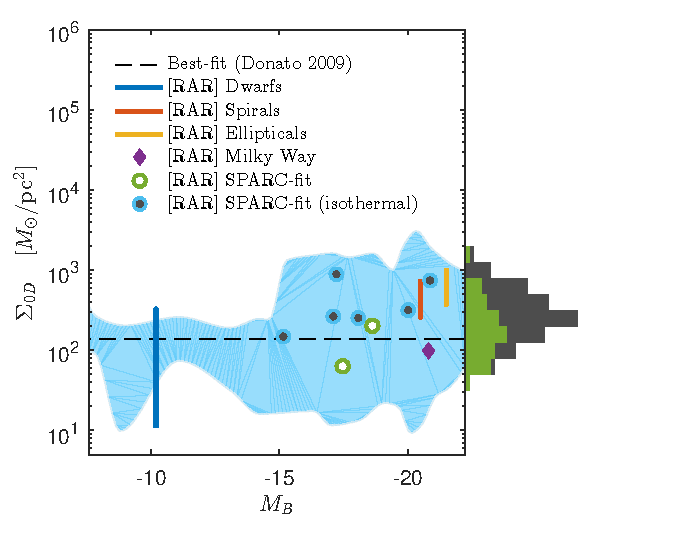
\includegraphics[width=\hsize]{\ROOTPATH/fig.pdf}
	\caption{$\chi^2$ profiles for DDO161. This galaxy is characterized through a rising rotation curve with a clear turning point. This \textit{deficit} of information in the outer halo region makes is difficult to favor either extended (isothermal-like) or contracted halos. All solutions are suitable for fitting well the rotation curve with a rather small change in the $\chi^2$ value. Solutions with lower $W_0$ values, corresponding to cuspy halos, are ruled out according to this analysis. With caution has to be taken the local minimum for relatively low $W_0$ values. This best-fit depends highly on the inner data points which are usually poorly constraint.}%
	\label{fig:DDO161:deep-chi2}%
\end{figure*}